\paragraph\
  Flow monitoring protocols like NetFlow\cite{NetFlow} and sFlow\cite{sFlow} can provide   important information about traffic that passes through a network. However contemporary  computer networking is out-spacing out ability to monitor them efficiently. As data 
  centers are getting virtualized with virtual software switches and scaling to thousands  of node, it is our immediate requirement to have monitoring system  that can scale 
  efficiently. There are few solutions that provide some methods to have scalable flow 
  monitoring in data center networks.
  
  \section{EMC2\cite{emc2}} 
  \paragraph\
    Edge Monitoring and Collection for Cloud (EMC2) is a scalable network 
    wide monitoring service for data centers. EMC2 stays inside host computer  to monitor
    virtual switches. Monitoring at virtual switch is scalable due to its 
    distributed nature.
    
  \subsection{Architecture}
    Figure 1.1 shows the architecture of EMC2.
    \begin{figure}[htb]
          \centering
          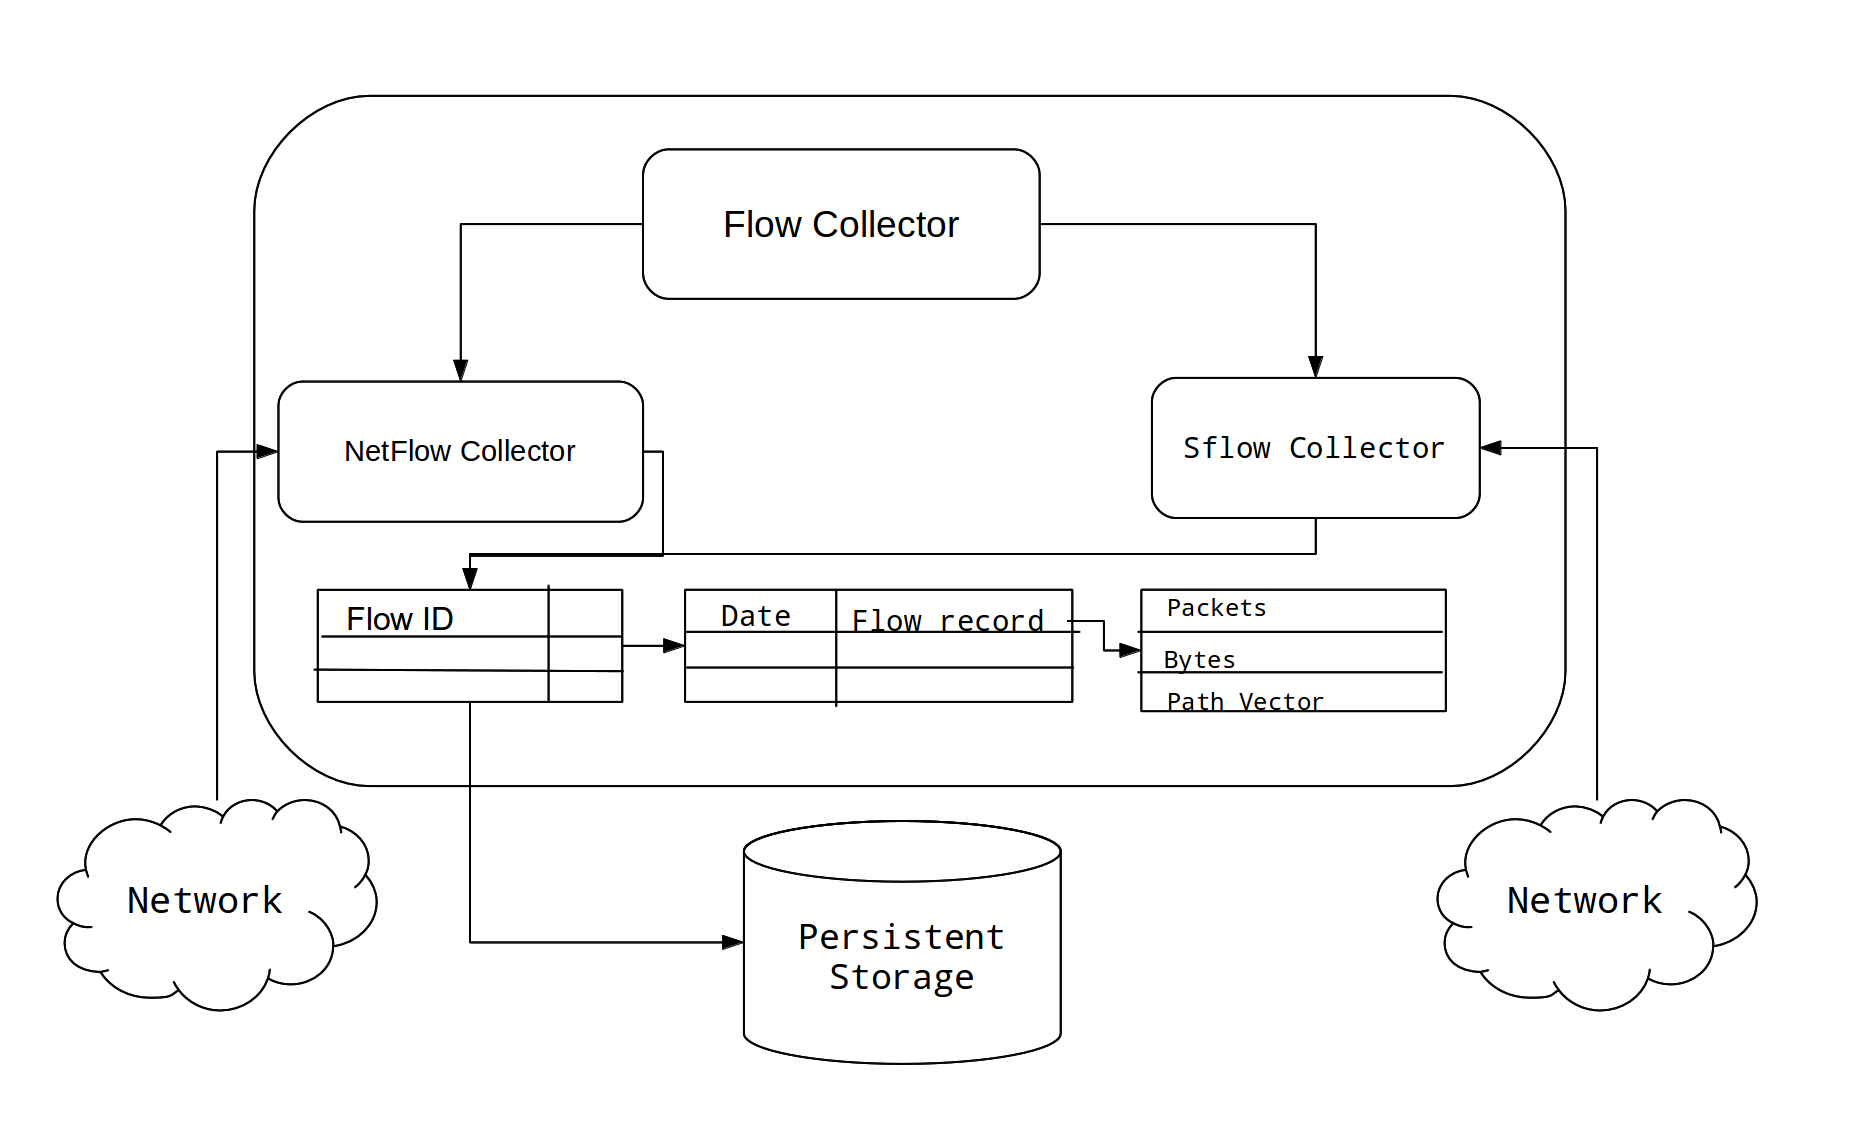
\includegraphics[scale=1]{emc2.png}
          \caption{Architecture of EMC2.} 
    \end{figure}
    
  \subsection{Modules}
  \paragraph\
    EMC2 is a multi-threaded application that contains following modules
    \begin{itemize}
     \item Flow-Table : Flow-Table is in-memory 2-level hash table.
     \item NetFlowParser : It parse NetFlow datagrams and update Flow-Table.
     \item sFlowParser : Its parse sFlow datagrams and update Flow-Table.
     \item NetFlowCollector : It accept NetFlow datagrams and create parser thread upon receiving NetFlow datagrams.
     \item sFlowCollector : It does the same task like NetFlowCollector for sFlow datagrams.
     \item FlowCollector : It invoke two thread, NetFlowCollector and sFlowCollector for accepting flow datagrams.
     
    \end{itemize}


    \subsubsection{Flow-Table}
      \paragraph\
	Flow-Table is a 2-level in-memory hash table. Layer-3 source and destination address forms Flow-ID that acts as 
	primary key for in-memory hash table. Flow-ID maps to another hash table where timestamp is the key and flow 
	record is value. Flow record contains number of packets, number of bytes and optional path vector.
 
    \subsubsection{NetFlowParser/sFlowParser}
      \paragraph\
	NetFlowCollector/sFlowCollector creates these two parser threads upon receiving a NetFlow/sFlow datagram.
	Parser threads parse the datagram and update the Flow-Table. Parser threads also performs two important
	tasks:

	\begin{itemize}
	 \item Deduplication.
	 \item Data rate prediction in presence of sampling.
	\end{itemize}
   
   \paragraph{Deduplication:}
       Deduplication avoids duplicate flow records to be added in Flow-Table. It uses the following algorithm.
       
     \begin{algorithm}[H]
        \caption{Detect Duplicate Flow}
	\label{alg1}

	\begin{algorithmic}
	  \IF{$flow-ID$ not exist}

	      \STATE add flow to the flow table.
	      \RETURN 

	  \ELSE 

	      \IF {Same exporter}
		  \STATE update the flow table.
		  \RETURN 

	      \ELSE

	        \STATE report duplicate flow.
	        \STATE update path vector.
	        \RETURN 

	      \ENDIF

	  \ENDIF

	\end{algorithmic}

       \end{algorithm}

    \paragraph{Data Rate Prediction in Presence of Sampling:}
       Sampling rate is specified in flow datagrams. Parser thread predict data rate by multiplying  sampling
       rate with length of the packet.
    
    \subsubsection{NetFlowCollector/sFlowCollector}
      NetFlowCollector/sFlowCollector are collector thread that waits for new NetFlow or sFlow datagrams and
      spawn a new NetFlowParser/sFlowParser thread upon receiving a datagram.
      
    \subsection{Advantages and Limitations}
    Claimed Advantages of EMC2 

    \begin{itemize}
     \item Scalable monitoring as EMC2 monitors host Vswitches which are distributed in nature. 
    \end{itemize}
    
    Disadvantages are
    
     \begin{itemize}
      \item Lack of scalable storage.
      \item Centralized monitoring will be difficult as it requires to fetch from distributed flats files.
     \end{itemize}
   \section{Scalable Internet Traffic Measurement and Analysis with Hadoop\cite{Lee}}
   